\documentclass[11pt]{report}

\usepackage[a4paper,top=3cm,bottom=3cm,left=3.5cm,right=3cm,marginparwidth=1.75cm,headheight=22pt]{geometry}
\usepackage[T1]{fontenc}
\usepackage[utf8]{inputenc}
\usepackage{mathptmx}
\usepackage{amsmath}
\usepackage{graphicx}
\usepackage{booktabs}
\usepackage{array}
\usepackage{tabularx}
\usepackage[labelfont=bf, textfont=bf]{caption}
\usepackage{setspace}
\usepackage[nottoc,notlot,notlof]{tocbibind}
\usepackage{fancyhdr}
\usepackage[numbers]{natbib}
\usepackage[colorlinks=true,linkcolor=black,citecolor=black,urlcolor=blue]{hyperref}

\setlength{\parindent}{0pt}
\setlength{\fboxrule}{0.5pt}
\pagestyle{plain}
\fontdimen2\font=0.5em

\fancypagestyle{plain}{
    \fancyhf{}
    \fancyhead[R]{\bf \small \textsl{\nouppercase{\leftmark}} \vspace{0.1in}}
    \fancyfoot[R]{\thepage}
    \renewcommand{\headrulewidth}{2pt}
}
\urlstyle{same}

\newcommand{\reporttitle}{Network Intrusion Detection Comparison Study}
\newcommand{\reportsubtitle}{A Final Project Report}
\newcommand{\coursename}{CSCC11 Winter 2026}
\newcommand{\institutionname}{University of Toronto Scarborough}
\newcommand{\reportdate}{April 2026}

\begin{document}

\hypersetup{pageanchor=false}
\pagenumbering{gobble}
\begin{titlepage}
\centering
\vspace*{0.6in}

{\fontsize{18}{18}\selectfont \textbf{\MakeUppercase{\reporttitle}} \par}
\vspace{0.55in}

{\fontsize{14}{14}\selectfont \textbf{\reportsubtitle} \par}
\vspace{0.25in}
{\fontsize{13}{13}\selectfont \textit{Submitted by} \par}
\vspace{0.25in}

{\fontsize{15}{15}\selectfont \textbf{Joshua Antonio Crisologo} \par}
\vspace{0.08in}
{\fontsize{15}{15}\selectfont \textbf{Albery Hyunh} \par}
\vspace{0.08in}
{\fontsize{15}{15}\selectfont \textbf{Daniel Venistan} \par}
\vspace{0.08in}
{\fontsize{15}{15}\selectfont \textbf{Nethenal Woubishet Reta} \par}
\vspace{0.55in}

{\fontsize{13}{13}\selectfont
\textit{in partial fulfillment of the course project requirements for} \par}
\vspace{0.18in}
{\fontsize{15}{15}\selectfont \textbf{\coursename} \par}
\vspace{0.6in}

{\fontsize{13}{13}\selectfont \textbf{Department of Computer and Mathematical Sciences} \par}
\vspace{0.08in}
{\fontsize{15}{15}\selectfont \textbf{\institutionname} \par}
\vspace{0.8in}

{\Large \textbf{\reportdate}}
\end{titlepage}
\newpage


\begin{titlepage}
\begin{center}
\vspace*{0.5in}
{\Large \textbf{ABSTRACT}}
\end{center}

\begin{spacing}{1.3}
\setlength{\parskip}{0.22in}

Short dummy text goes here. Write a brief summary of the problem, methods, and main findings.

\textbf{Keywords:} Short dummy text goes here.
\end{spacing}
\end{titlepage}
\newpage


\clearpage
\hypersetup{pageanchor=true}
\pagenumbering{roman}
\renewcommand*\contentsname{\centering Table of Contents}
\tableofcontents
\newpage

\pagenumbering{arabic}
\chapter{Introduction}
\begin{spacing}{1.5}
\setlength{\parskip}{0.3in}

Machine learning has become an increasingly important component of modern cybersecurity systems because network traffic is too large, fast-moving, and complex to monitor effectively by manual inspection alone. One particularly important application is network intrusion detection, where the goal is to distinguish benign activity from malicious behaviour as early and reliably as possible. In practice, such systems must balance two competing demands: they should detect as many attacks as possible, but they should also avoid generating so many false alarms that analysts are overwhelmed. This makes intrusion detection a natural and practically important machine learning problem.

\section{Problem Statement}
In this project, we study the UNSW-NB15 network intrusion dataset as distributed through Kaggle \cite{kaggle_unsw_nb15}. The dataset contains modern normal network traffic together with nine attack categories: Fuzzers, Analysis, Backdoors, DoS, Exploits, Generic, Reconnaissance, Shellcode, and Worms. In the version used for this project, each record is represented as a tabular network-flow example with 49 original features and a class label \cite{kaggle_unsw_nb15}.

Our task is a binary classification problem: given a network-flow record, predict whether it corresponds to normal activity (label 0) or an attack (label 1). The main research question of this project is:

\textit{How do classical machine learning models and a more advanced ensemble method compare on modern tabular network intrusion detection data, and which model provides the best overall trade-off between predictive performance, robustness, and practical usefulness?}

More specifically, we investigate whether tree-based and neural-network approaches meaningfully outperform Logistic Regression as a simple linear baseline, and whether the advanced model offers a convincing practical improvement over the standard methods covered in class.

\section{Motivation}
This problem is important because false negatives and false positives have very different operational costs. A false negative means malicious traffic is allowed to pass undetected, which can lead to system compromise, data loss, or service disruption. A false positive, on the other hand, incorrectly flags benign traffic as malicious and can create alert fatigue for analysts if it happens too frequently. A useful intrusion detection model must therefore be evaluated not only by overall accuracy, but also by its ability to separate attack traffic from normal traffic under a realistic thresholding and evaluation framework.

The UNSW-NB15 dataset is well suited to this goal because it is more modern than many older intrusion-detection benchmarks and includes both normal traffic and diverse attack behaviours \cite{kaggle_unsw_nb15}. It therefore provides a meaningful setting in which to test how different model families behave on structured cybersecurity data.

\section{Existing Approaches and Our Direction}
Existing machine learning approaches to intrusion detection span several families, including supervised linear models, tree ensembles, and neural networks. A recent survey by Pinto et al. notes that supervised learning remains a dominant approach in practical IDS research because it can achieve strong detection performance on labeled attack data, while more complex approaches such as deep learning and ensemble methods are increasingly used when the goal is to model nonlinear behavior and richer feature interactions \cite{ids_survey_ci}. On the UNSW-NB15 dataset specifically, Kasongo and Sun compared several supervised models, including Logistic Regression, k-nearest neighbors, support vector machines, artificial neural networks, decision trees, and Naive Bayes, together with a feature-selection pipeline \cite{kasongo_sun_unsw}. More recently, Yin et al. proposed an MLP-based intrusion detection method for UNSW-NB15 that combines information gain, random forest ranking, and recursive feature elimination to improve feature selection before neural classification \cite{yin_igrf_rfe}.

Our direction is more comparative and course-aligned than proposing a new feature-selection or neural architecture. We evaluate four representative models on the same binary intrusion-detection task under a shared preprocessing and evaluation pipeline: Logistic Regression, Multi-Layer Perceptron, Random Forest, and XGBoost. Logistic Regression, MLP, and Random Forest serve as the three core models from the course, while XGBoost is our advanced method. We selected XGBoost because it extends lecture ideas about decision trees, ensembles, and optimization into a stronger boosted-tree framework, and because gradient-boosted trees are widely recognized as strong methods for structured tabular classification \cite{xgboost_paper}. This gives us a clear way to test whether a more sophisticated ensemble delivers a practical improvement over the standard baselines on UNSW-NB15 without changing the problem definition or evaluation setup.

\end{spacing}
\newpage

\chapter{Data Collection, Preprocessing, and Representation}
\begin{spacing}{1.5}
\setlength{\parskip}{0.3in}

We use the UNSW-NB15 network intrusion dataset as provided through Kaggle \cite{kaggle_unsw_nb15}. The original records contain 49 traffic attributes together with the categorical attack type and a binary label indicating whether a flow is normal or malicious. Following the rest of our project, we study the binary intrusion-detection task: predict Normal ($0$) versus Attack ($1$) for each network flow.

\section{Dataset Description}
The provided data come as two official CSV splits. Our preprocessing pipeline first removes duplicate flows from each split, then constructs model-ready datasets used throughout the model notebooks. Table~\ref{tab:data-split-summary} summarizes the final sizes consumed by the experiments. The training matrix used for hyperparameter tuning and model fitting contains 55{,}945 examples, while the held-out test matrix contains 107{,}740 examples. After preprocessing, each model sees 58 input features plus the binary label: 21 one-hot encoded categorical indicators and 37 numerical features.

\begin{table}[htbp]
    \centering
    \caption{Final model-ready dataset sizes after duplicate removal.}
    \label{tab:data-split-summary}
    \begin{tabularx}{\linewidth}{l c c c}
        \toprule
        Split & Total Rows & Normal & Attack \\
        \midrule
        Training & 55{,}945 & 34{,}206 (61.1\%) & 21{,}739 (38.9\%) \\
        Test & 107{,}740 & 51{,}890 (48.2\%) & 55{,}850 (51.8\%) \\
        \bottomrule
    \end{tabularx}
\end{table}

The feature space contains three categorical variables, \texttt{proto}, \texttt{service}, and \texttt{state}, together with 37 numerical traffic statistics such as packet counts, byte counts, delays, TCP timing features, and connection-level counters. This mixture of sparse categorical information and heavy-tailed numerical measurements is what drives the rest of the preprocessing design.

\section{Data Exploration}
Our exploratory analysis focused on three questions: how skewed the numerical variables are, how concentrated the categorical distributions are, and whether strong linear dependencies exist among the numerical features. These diagnostics were produced in the preprocessing notebook and guided every transformation used later in the model pipeline.

Figure~\ref{fig:skewness-log1p} shows the 14 most strongly right-skewed numerical features before and after a $\log(1+x)$ transformation. Variables such as \texttt{sload}, \texttt{dload}, \texttt{sbytes}, \texttt{dbytes}, \texttt{rate}, \texttt{sjit}, and \texttt{djit} span several orders of magnitude, with most observations compressed near zero and a small number of extremely large outliers. On the raw scale, these distributions are difficult to inspect visually and would dominate any scale-sensitive model; on the log scale, the structure becomes much more interpretable.

\begin{figure}[htbp]
    \centering
    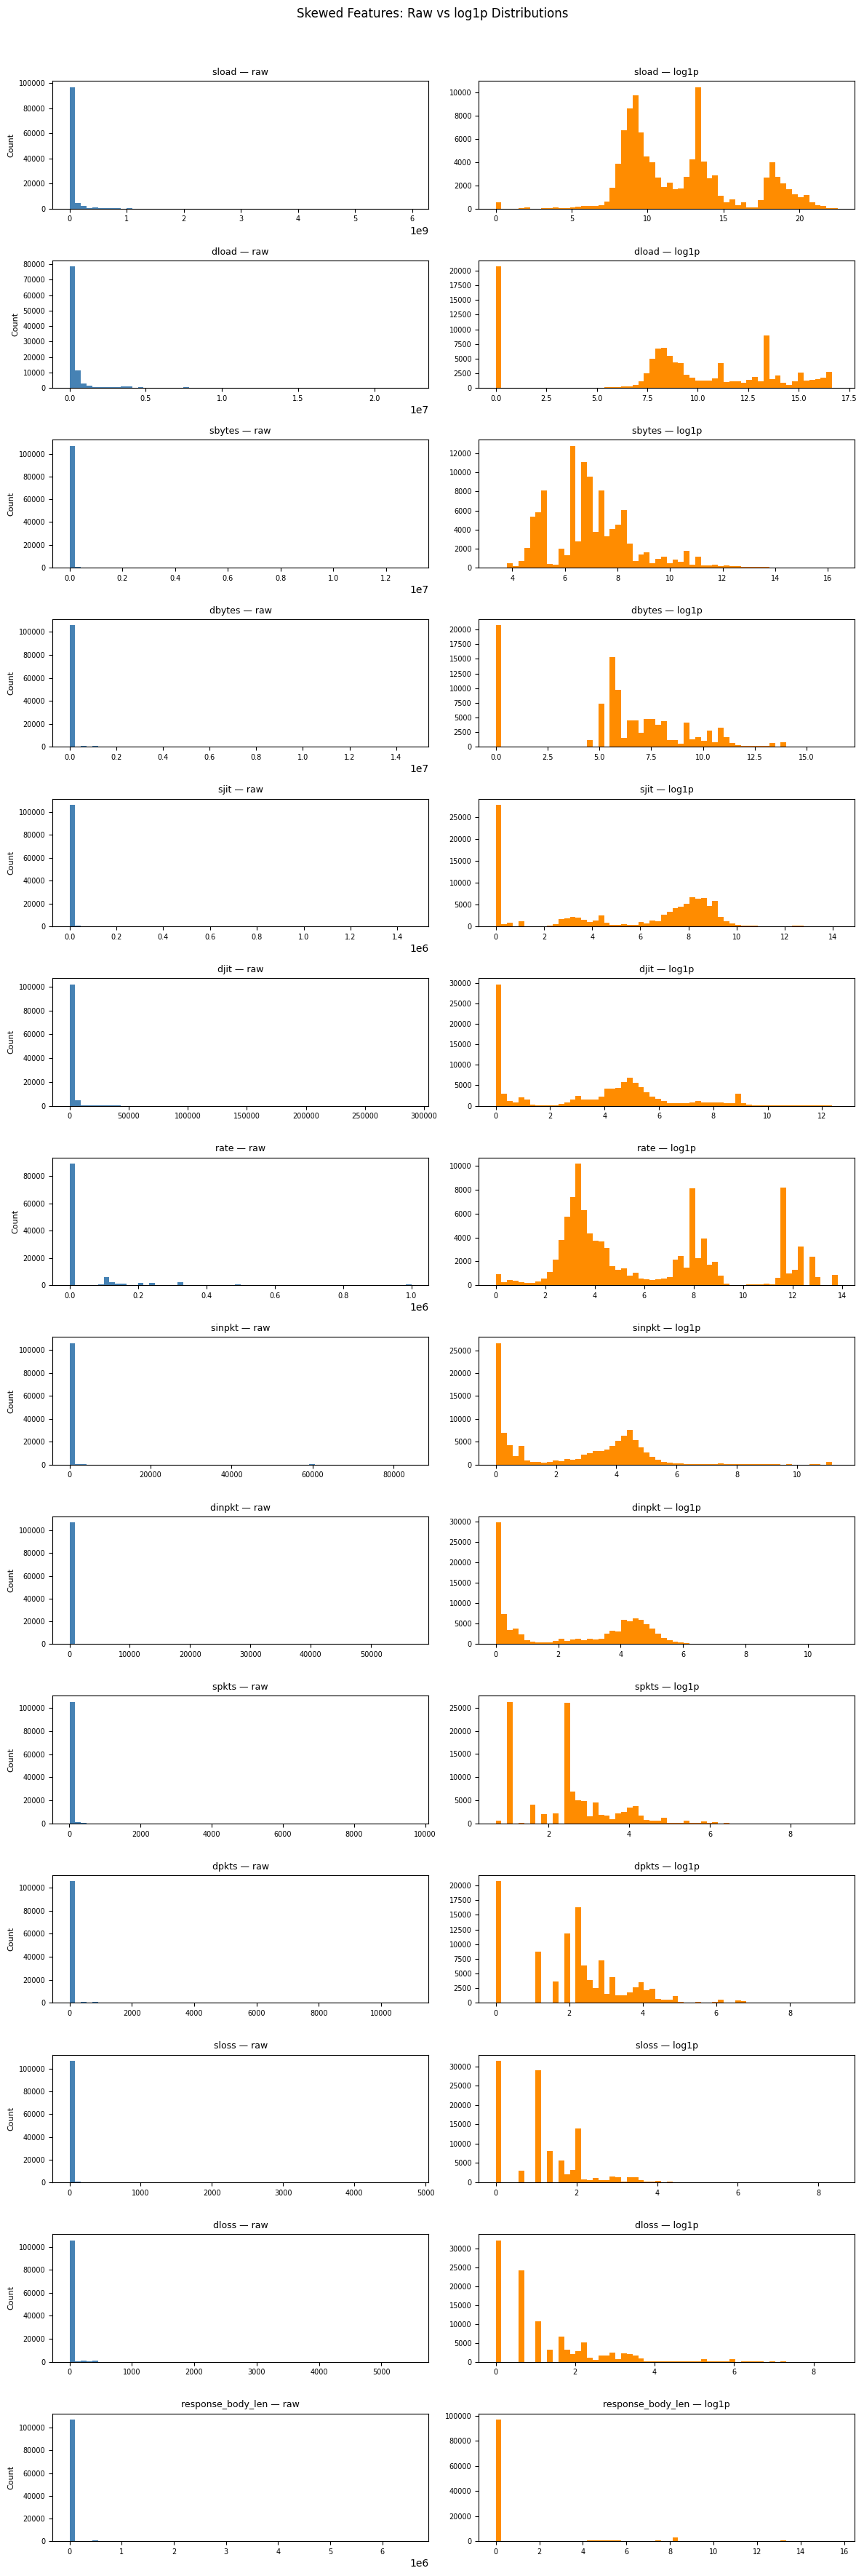
\includegraphics[width=\linewidth,height=0.3\textheight,keepaspectratio]{../report/plots/skewness_plots.png}
    \caption{Raw versus $\log(1+x)$ distributions for the heavily skewed numerical features identified during exploratory analysis.}
    \label{fig:skewness-log1p}
\end{figure}

The categorical exploration in Figure~\ref{fig:categorical-buckets} shows that only a small number of protocol, service, and state values appear frequently. In the raw data, \texttt{proto} has 131 distinct values, but only six of them occur often enough to be informative at scale. The same concentration pattern appears in \texttt{service} and \texttt{state}. This justified collapsing rare categories into an \texttt{other} bucket before one-hot encoding so that the linear and neural models would not be forced to learn from dozens of nearly empty indicator columns.

\begin{figure}[htbp]
    \centering
    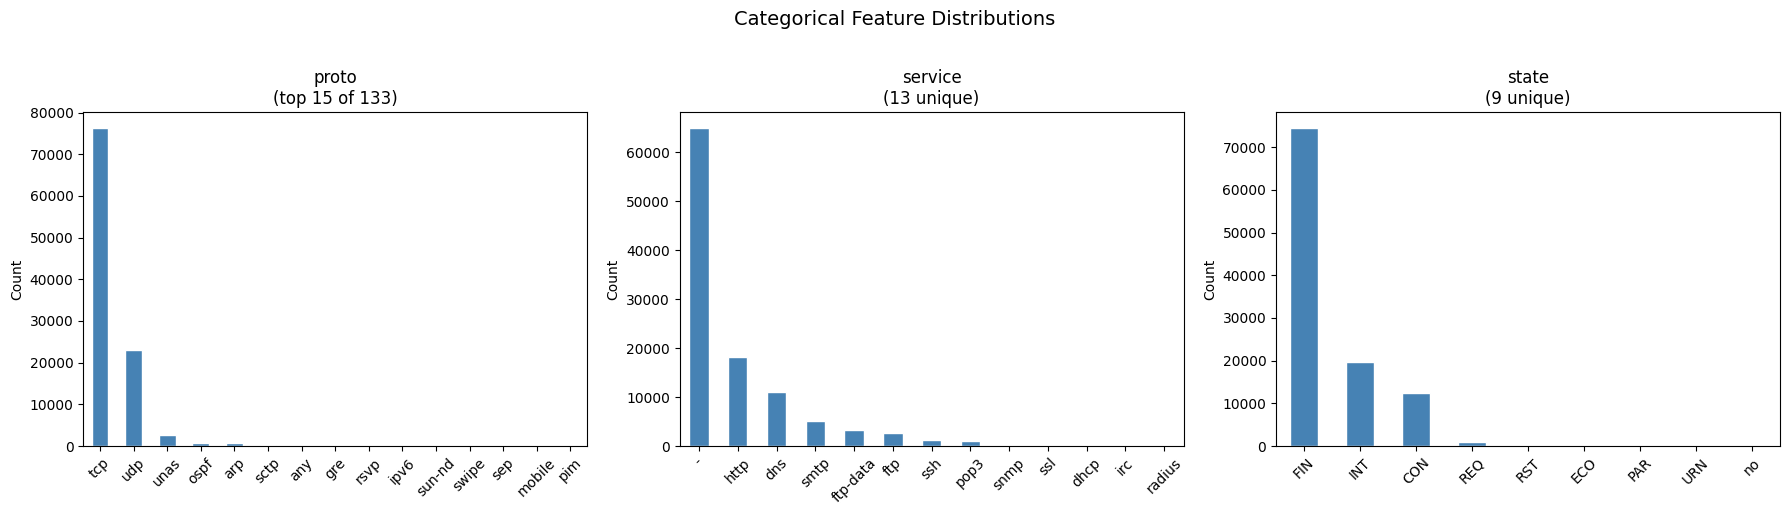
\includegraphics[width=\linewidth,height=0.26\textheight,keepaspectratio]{../report/plots/categorical_plots.png}
    \caption{Frequency distributions of the bucketed categorical features used in the final preprocessing pipeline.}
    \label{fig:categorical-buckets}
\end{figure}

Finally, we examined the numerical correlation structure. The correlation heatmap in Figure~\ref{fig:correlation-heatmap} reveals several highly correlated pairs, especially among throughput- and packet-volume-related variables. We kept these features rather than dropping them aggressively because the tree-based models are robust to correlated inputs and the Logistic Regression baseline can still benefit from keeping distinct but related traffic statistics when regularization is used.

\begin{figure}[htbp]
    \centering
    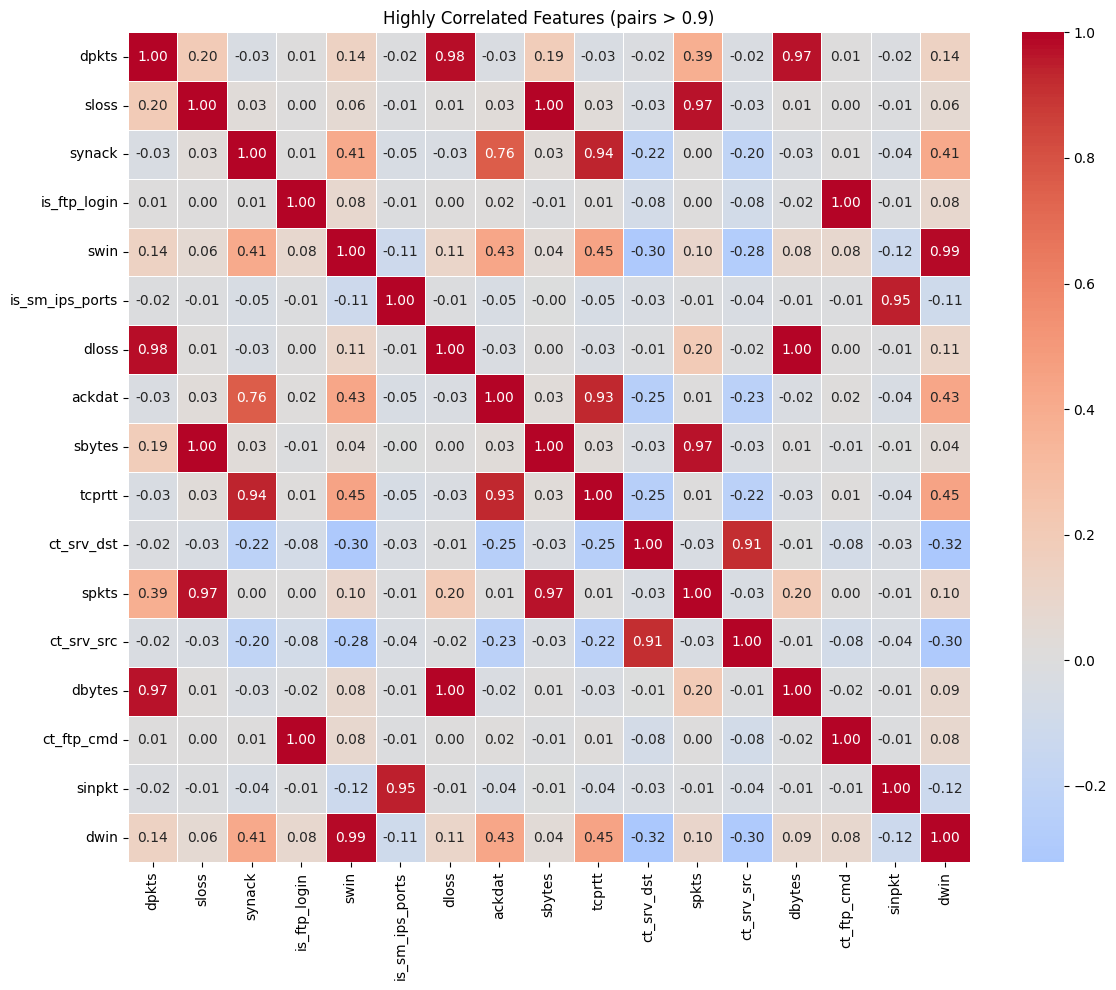
\includegraphics[width=\linewidth,height=0.3\textheight,keepaspectratio]{../report/plots/correlation-heatmap.png}
    \caption{Correlation heatmap over the numerical features used during exploratory analysis.}
    \label{fig:correlation-heatmap}
\end{figure}

\section{Data Cleaning}
The preprocessing code begins by verifying that the dataset contains no missing values; the training split passes this check without requiring imputation. We then remove duplicate rows using all columns except \texttt{id}. This step is important because repeated flows would otherwise inflate downstream metrics and make the held-out evaluation less trustworthy.

We also remove four columns before model fitting:
\begin{itemize}
    \item \texttt{id}, because it is only a row identifier and carries no predictive signal;
    \item \texttt{attack\_cat}, because our task is binary intrusion detection rather than multi-class attack-type prediction;
    \item \texttt{stcpb} and \texttt{dtcpb}, because these TCP base sequence numbers behave like connection-specific identifiers rather than stable behavioural features.
\end{itemize}

\section{Feature Engineering}
The final feature engineering pipeline has three main stages. First, the categorical variables are bucketed by frequency and then one-hot encoded. For \texttt{proto}, we retain \texttt{tcp}, \texttt{udp}, \texttt{unas}, \texttt{arp}, \texttt{ospf}, and \texttt{sctp}. For \texttt{service}, we retain \texttt{-}, \texttt{http}, \texttt{dns}, \texttt{smtp}, \texttt{ftp-data}, \texttt{ftp}, \texttt{ssh}, and \texttt{pop3}. For \texttt{state}, we retain \texttt{FIN}, \texttt{INT}, \texttt{CON}, and \texttt{REQ}. All remaining values are mapped to \texttt{other}. This produces 21 binary indicator columns in total and keeps the categorical representation compact enough for Logistic Regression and the MLP.

Second, we apply $\log(1+x)$ to 14 heavily skewed numerical variables, including load, byte-count, jitter, packet-count, and loss features together with \texttt{response\_body\_len}. We use $\log(1+x)$ instead of $\log(x)$ because many flows have zero values and the shifted transform remains well-defined at zero.

Third, for models that are sensitive to feature scale, we standardize the numerical variables using \texttt{StandardScaler}. The scaler is fit only on the training split and then reused to transform the held-out test split, preventing leakage from the test distribution into the fitted means and variances. The same leakage-avoidance rule is used for categorical encoding: the one-hot column set is learned on the training split and then reindexed on the test split so that unseen or missing categories are handled consistently.

\section{Data Representation and Splits}
We maintain two model-specific representations derived from the same cleaned data:
\begin{itemize}
    \item \textbf{Scaled matrix (\texttt{df\_model})}: 21 one-hot encoded categorical indicators, 14 log-transformed and scaled skewed numerical features, and 23 additional scaled numerical features. This representation is used by Logistic Regression and the Multi-Layer Perceptron.
    \item \textbf{Tree matrix (\texttt{df\_model\_tree})}: the same 21 one-hot encoded indicators combined with the 37 raw numerical features, without standardization. This representation is used by Random Forest and XGBoost, which are largely invariant to monotone rescaling.
\end{itemize}

Both matrices therefore contain 58 predictors plus the label column. To keep preprocessing consistent between training and evaluation, the fitted scaler, one-hot column definitions, and column lists are serialized and reused when transforming the held-out split.

For hyperparameter tuning, we do not carve out a separate validation set from the saved training matrix. Instead, each model uses \texttt{RandomizedSearchCV} with 3-fold cross-validation on the training split, scored by ROC-AUC. Concretely, the 55{,}945-row training matrix is partitioned into three folds for each sampled hyperparameter configuration, while the 107{,}740-row test matrix remains untouched until the final model evaluation. This setup lets us tune models efficiently while preserving a completely held-out dataset for the final comparison study.

\end{spacing}
\newpage

\chapter{Model Comparison Study}
\begin{spacing}{1.0}
\small

\section{Model Descriptions and Motivations}

\subsection{Logistic Regression}

Logistic regression is a linear model that uses a linear combination of its inputs to model the log-odds of the positive class and outputting a probability using the sigmoid function. More specifically, it uses the formula $p = \sigma(w^T x + b)$ to calculate these odds, and is optimized by minimizing cross-entropy loss using gradient descent. To prevent overfitting, the model also supports L1, L2, and elastic-net regularization (L1 sparsifies coefficients, L2 shrinks them, and elastic net combines both). It is a popular baseline for classification problems, especially on tabular data due to its simplicity, accurate predictions, and interpretability. 

We chose the logistic regression model as we want to use it as a baseline for predictive power in our dataset. Since it is one of the simplest models, it is the best reference for judging if the more complex models perform well. We believe that this model would fit well on the UNSW-NB15 dataset due to its tabular data with some correlated features, where logistic regression's optimization and regularization shine.
\subsection{Multi-Layer Perceptron (MLP)}

Multi-Layer Perceptron (MLP) is a supervised learning algorithm and is also known as a modern feedforward neural network. It consists of fully connected dense layers that transform input data from one dimension to another. These dense layers are made up of neurons with nonlinear activation functions, which allow the network to model complex patterns and distinguish data that is not linearly separable, and can be used for both classification or regression.

The basic workflow of the MLP can be simplified via forward propagation, loss functions, backpropagation and optimization. Each neuron in a hidden or output layer computes a weighted sum of its inputs: $z = \sum_i w_i x_i + b$ where \(x_i\) is the input value, \(w_i\) is the corresponding weight, and \(b\) is the bias term. After calculating \(z\), the neuron applies an activation function to produce its output. When we reach the output layer, the model's error is calculated using a loss function — binary cross-entropy for classification, or mean squared error (MSE) for regression. Once the loss is computed, we calculate the gradient of the loss with respect to each weight, which is then propagated backward through the network layer by layer, allowing us to update the weights in a way that reduces the loss in future predictions. To prevent overfitting, MLPs commonly use regularization techniques such as dropout, which randomly deactivates a fraction of neurons during training, and L2 regularization (weight decay), which penalizes large weights in the loss function to encourage simpler, more generalizable models.

We selected the MLP for two reasons: First, MLP benefits directly from the scaled and log-transformed preprocessing applied to our dataset, as gradient-based optimization converges more effectively on normalized inputs, which is an advantage that tree-based models like XGBoost and Random Forest do not require. Second, MLP builds naturally on what we learned in lecture about neural networks and gradient descent, making it a fitting and well-motivated addition to our model comparison. 
\subsection{Random Forest}

Random Forest is a tree-based ensemble algorithm that builds a large number of decision trees and, in classification, determines a label using majority vote. Each tree is trained with a sample of the training data (bagging) with only a random subset of features to reduce variance/overfitting, and an ensemble improves prediction power compared to a single tree. Because trees are trained independently in parallel, any form of boosting is not used, which differs from XGBoost. This trades the bias-reduction benefits of boosting for lower sensitivity to noise, since errors are averaged out than sequentially built upon.

We selected Random Forest as a tree-based baseline for three main reasons. Firstly, Random Forest is one of the most well-established and widely-used algorithms for tabular classification tasks, which makes it a competitive reference against more complex models (XGBoost, MLP). Secondly, we wanted to evaluate whether boosting (XGBoost) meaningfully outperforms bagging (Random Forest) on this specific dataset and problem setting. Lastly, Random Forest extends our learning from lecture concepts such as decision trees and ensembles, making it a motivated choice along the more advanced models.

\subsection{XGBoost}

XGBoost stands for Extreme Gradient Boosting and is an ML framework that provides a gradient-boosted decision tree (GBDT) implementation that is scalable and distributed. Similar to Random Forest and the topics we learned in class, a GBDT is an ensemble decision tree learning algorithm. RF builds decision trees independently in parallel via bagging, while XGBoost uses gradient boosting to build a new tree that learns from the previous tree's ``mistakes.'' These errors are represented by setting an objective function and minimizing it using the gradient descent algorithm to create the targeted outcome for the next model.

XGBoost extends gradient boosting through its use of both the first and second order gradient statistics (gradient and Hessian) on the loss function to find the optimal score, leading to fast convergence and a better tree structure. The objective is also regularized using both L1 (lasso) and L2 (ridge) regularization in the objective function itself to decrease overfitting. It also takes advantage of shrinkage, which scales new weights by a factor after a step of boosting and thus ensures no one tree has too much influence, and row/column subsampling, which introduces randomness similar to the random forest algorithm. It also uses sparsity-aware splitting to handle missing/sparse features, and a weighted quantile sketch to find efficient splits, making it robust and scalable.

We selected XGBoost as the advanced/novel model in our project for three main reasons. Firstly, XGBoost is widely known as the SOTA ML when it comes to classification problems on tabular data. We wanted to gauge XGBoost's performance on this set of tabular data with a large number of features. Secondly, we wanted to compare tree-based models vs MLP on tabular data (with logistic regression as a baseline). Neural networks are rising in popularity, however, we wanted to show that deep learning approaches may not be the most optimal, as we found that tree-based models outperformed it in a tabular setting.  Lastly, XGBoost extends many concepts covered in lecture (decision trees, ensembles, gradient descent), making it a motivated choice.

\section{Evaluation Setup}
All models were trained on the same processed training split
and evaluated on the same test split, with 3-fold cross-validation on
the training data for model selection. \textbf{Metrics:} ROC-AUC was used as the metric for
cross-validation as it measures the model's ability to rank positives above negatives (handling imbalance) without fixing a decision
threshold. Precision, recall, and F1 were then reported on the test set because
a robust model must balance false alarms against missed attacks.
\textbf{Tuning:} Model hyperparameters were tuned with RandomizedSearchCV using search
spaces that cover simpler and more expressive settings without
becoming computationally excessive. \textbf{Threshold analysis:} After fitting
the best cross-validated model, thresholds from 0.01 to 0.99 were swept and
the threshold maximizing attack-class F1 was selected. The goal was to see the optimal threshold that would
maximize each model's ability to distinguish between false and real attacks. Additionally, the tuned predictions were also joined back to the
raw \texttt{attack\_cat} labels to find out which attack category models struggle to classify.

\section{Model and Tuning Summary}
\begin{table}[htbp]
    \centering
    \footnotesize
    \setlength{\tabcolsep}{3pt}
    \caption{Models, motivations, and tuning spaces used in the comparison.}
    \label{tab:model-tuning-summary}
    \begin{tabularx}{\linewidth}{>{\raggedright\arraybackslash}p{2.2cm} X X}
        \toprule
        Model & What it is / why selected & Hyperparameters tried and best configuration \\
        \midrule
        Logistic Regression &
        Linear probabilistic classifier; selected as the most interpretable
        baseline and as a reference point for judging whether nonlinear models
        add meaningful predictive value. &
        Tried C on a log-uniform range from 1e-3 to 1e3, penalties l1, l2,
        and elasticnet, class\_weight values None and balanced, and elastic-net
        l1\_ratio from 0.1 to 0.9 using saga with max\_iter = 2000. Best:
        penalty = elasticnet, C = 897.9856, l1\_ratio = 0.3434,
        class\_weight = None. \\
        \addlinespace[0.3em]
        MLP &
        Feedforward neural network; selected to test whether a flexible
        nonlinear dense model improves over the linear baseline. &
        Tried
        hidden\_layer\_sizes from single- and multi-layer layouts between
        (32) and (256,128,64,32), activation values relu and tanh,
        learning\_rate\_init values 1e-2, 1e-3, 5e-4, 3e-4, and 1e-4, alpha
        values 1e-4, 1e-3, 1e-2, 0.1, and 1.0, and batch\_size values 32, 64,
        128, and 256. Best: hidden\_layer\_sizes = (128,64),
        activation = tanh, learning\_rate\_init = 0.01, alpha = 0.01,
        batch\_size = 128. \\
        \addlinespace[0.3em]
        Random Forest &
        Bagged ensemble of decision trees; selected as a strong tabular
        baseline that captures nonlinear feature interactions and is robust to
        feature scaling details. &
        Tried n\_estimators values 100, 200, 300, and 500; max\_depth values
        None, 10, 20, 30, and 40; min\_samples\_split values 2, 5, 10, and 20;
        min\_samples\_leaf values 1, 2, 4, and 8; max\_features values sqrt,
        log2, 0.3, and 0.5; and bootstrap values True and False. Best:
        n\_estimators = 300, max\_depth = 10, min\_samples\_split = 20,
        min\_samples\_leaf = 4, max\_features = 0.3, bootstrap = True. \\
        \addlinespace[0.3em]
        XGBoost &
        Gradient-boosted tree ensemble; selected as the most advanced model in
        the study and the one most likely to exploit structured tabular
        patterns in intrusion data. &
        Tried n\_estimators values 200, 300, 500, 700, and 1000; max\_depth
        values 3, 4, 5, 6, and 8; learning\_rate values 0.01, 0.05, 0.1, and
        0.2; subsample and colsample\_bytree values 0.6, 0.7, 0.8, and 1.0;
        min\_child\_weight values 1, 3, and 5; gamma values 0, 0.1, 0.3, and
        0.5; reg\_alpha values 0, 0.1, 0.5, and 1.0; and reg\_lambda values
        0.5, 1.0, 2.0, and 5.0. Best: n\_estimators = 1000, max\_depth = 4,
        learning\_rate = 0.01, subsample = 0.7, colsample\_bytree = 0.8,
        min\_child\_weight = 1, gamma = 0.1, reg\_alpha = 1.0,
        reg\_lambda = 2.0. \\
        \bottomrule
    \end{tabularx}
\end{table}

\section{Results Comparison}
\begin{table}[htbp]
    \centering
    \footnotesize
    \setlength{\tabcolsep}{3pt}
    \caption{Cross-model comparison on validation and test metrics.}
    \label{tab:model-comparison-good}
    \begin{tabularx}{\linewidth}{>{\raggedright\arraybackslash}p{2.2cm} c c c c X}
        \toprule
        Model & CV ROC-AUC & Test ROC-AUC & Best threshold & Tuned F1 & Takeaway \\
        \midrule
        Logistic Regression & 0.9435 & 0.9586 & 0.05 & 0.9080 & Most interpretable; weakest ranking performance, but competitive after threshold tuning. Highest Fuzzers recall across all models (0.9591). \\
        MLP & 0.9508 & 0.9549 & 0.83 & 0.8425 & Weakest tuned F1 among all four models; Fuzzers is by far its hardest category at 0.4475 recall. \\
        Random Forest & 0.9484 & 0.9729 & 0.04 & 0.9091 & Best test ROC-AUC overall; strong and consistent across attack families. \\
        XGBoost & 0.9601 & 0.9695 & 0.04 & 0.9154 & Best cross-validation ROC-AUC and best tuned F1; marginally behind Random Forest on held-out test ROC-AUC. \\
        \bottomrule
    \end{tabularx}
\end{table}

All four models improved after threshold tuning compared to the default 0.50
threshold. Logistic Regression improved from 0.7899 to 0.9080, Random Forest
from 0.8471 to 0.9091, XGBoost from 0.8466 to 0.9154, and MLP from 0.8067 to
0.8425. This confirms that the default threshold is too conservative for this
intrusion-detection setting and that the threshold sweep produced meaningfully
better operating points for attack detection.

The two tree-based models achieved the strongest overall scores. Random Forest
achieved the highest test ROC-AUC (0.9729), while XGBoost led on
cross-validation ROC-AUC (0.9601) and tuned F1 (0.9154). The gap between
them is small — 0.0034 on test ROC-AUC — and the two models produced
identical per-attack-category recall after threshold tuning: Fuzzers was the
hardest category for both at 0.6255 recall, followed by Analysis at 0.8812,
with all remaining categories at 0.9656 or higher and Worms reaching perfect
recall (1.0000). The close performance between Random Forest and XGBoost is
consistent with the nearly balanced class distribution in this dataset, which
limits the gradient signal that boosting can exploit.

Logistic Regression, despite being the simplest model, remained competitive
after tuning (F1 = 0.9080) and achieved the highest Fuzzers recall across all
four models at 0.9591, with Analysis being its weakest category at 0.9586.
This suggests Fuzzers may be more linearly separable than expected. MLP
achieved a test ROC-AUC of 0.9549 and a tuned F1 of 0.8425 — the lowest
among all four models — with Fuzzers being by far its hardest category at
only 0.4475 recall, the lowest Fuzzers recall across all models.

\end{spacing}
\newpage

\chapter{Originality and Future Work}
\begin{spacing}{1.3}

\section{Originality}

Short dummy text goes here. Explain how this project differs from prior work or standard baselines.

\section{Future Work}

One possible direction for future work would be to replace the scikit-learn \texttt{MLPClassifier} with a deep learning
framework such as PyTorch or Keras. While scikit-learn’s MLP is simple and sufficient for a baseline, it lacks several
important training features. It does not support dropout, a regularization technique that randomly deactivates neurons 
during training to reduce overfitting and improve generalization. It also lacks batch normalization, which stabilizes 
training by keeping activations consistent across layers — something that becomes increasingly important in deeper architectures.
Additionally, scikit-learn does not allow per-class or per-sample loss weighting, meaning the model cannot be directed to penalize
false negatives more heavily than false positives. In a cybersecurity context, this is a significant limitation since missing an
attack is typically far more costly than a false alarm. Switching to PyTorch or Keras would address all of these issues and open
the door to custom loss functions such as focal loss, which focuses training on hard-to-classify examples, as well as more advanced
learning rate strategies such as cosine annealing or warm restarts.

This is particularly relevant given that Fuzzers were the hardest attack type to detect across all models in this study, achieving
only 44.75\% recall in MLP and around 62\% in both tree-based models. A more expressive and configurable neural network trained with
focal loss could force the model to focus on these ambiguous samples rather than the easier categories it already handles well. 
Oversampling the Fuzzers class could help improve performance further. Interestingly, Logistic Regression achieved the highest
Fuzzers recall (95.91), suggesting the class may be more linearly separable than expected and that more complex models may be overfitting.
Future work could explore using Logistic Regression specifically for Fuzzers detection as part of an ensemble model.

Another promising direction is model ensembling or stacking. In this study, Logistic Regression, Random Forest, XGBoost, and MLP were
each evaluated independently, yet each model showed different strengths across attack categories. For example, Logistic Regression 
achieved the highest Fuzzers recall while tree-based models excelled on other categories. Rather than selecting a single best model,
a stacking approach could combine the predictions of all four models using a meta-learner, allowing the ensemble to exploit the 
complementary strengths of each classifier.

Finally, all models in this study were trained and evaluated exclusively on the UNSW-NB15 dataset, which was collected in a controlled
lab environment in 2015. This raises questions about how well these models would generalize to real-world traffic or more recent datasets
such as CIC-IDS2017. Since network traffic and attack patterns evolve over time, cross-dataset validation would be a valuable next step 
to better assess the true generalizability of these models.

\end{spacing}
\newpage

\chapter{Main Results and Conclusion}
\begin{spacing}{1.15}

\section{Main Results}
Table~\ref{tab:main-results-summary} summarizes the main results of the
comparison study. A consistent pattern across all four models is that the
default threshold of 0.50 was too conservative for this intrusion-detection
task. After threshold tuning, every model achieved a tuned attack-class F1
above 0.90, which shows that threshold selection was an important part of the
final evaluation.

\begin{table}[htbp]
    \centering
    \small
    \setlength{\tabcolsep}{4pt}
    \caption{Main results, strengths, and weaknesses of the compared models.}
    \label{tab:main-results-summary}
    \begin{tabularx}{\linewidth}{>{\raggedright\arraybackslash}p{2.2cm} c c X X}
        \toprule
        Model & Test ROC-AUC & Tuned F1 & Main strength & Main weakness \\
        \midrule
        Logistic Regression & 0.9586 & 0.9080 & Most interpretable model; after tuning it reached 0.98 attack recall and remained competitive as a simple linear baseline. & Lowest ROC-AUC of the four models and the most sensitive to threshold choice. \\
        MLP & 0.9693 & 0.9121 & Strong nonlinear baseline; achieved 0.99 attack recall after tuning and very strong recall on Analysis (0.9529) and Fuzzers (0.9849). & Less interpretable than the linear model and still weaker than the tree ensembles on ROC-AUC. \\
        Random Forest & 0.9736 & 0.9091 & Strong tabular baseline with robust performance on most attack families and near-perfect recall on Backdoor, Worms, and Reconnaissance. & Weakest family-level recall on Analysis and Fuzzers (both 0.8614), which limited its final tuned F1. \\
        XGBoost & 0.9761 & 0.9154 & Best overall model; highest validation ROC-AUC, highest test ROC-AUC, and highest tuned F1, with strong results across nearly all attack families. & Most complex and least interpretable model, with a larger tuning burden than the baselines. \\
        \bottomrule
    \end{tabularx}
\end{table}

The results show a clear hierarchy. Logistic Regression served as a strong
interpretable baseline, but its lower ROC-AUC indicates that a linear decision
boundary cannot capture all of the structure in the UNSW-NB15 features. The
MLP improved substantially over the linear baseline and performed especially
well after threshold tuning, showing that a nonlinear neural model can compete
on this task. However, the two tree-based ensemble models achieved the
strongest threshold-independent ranking performance, which suggests that the
dataset contains important nonlinear feature interactions that are well handled
by ensemble trees.

Per-attack-category analysis also reveals where the models struggle. Analysis
was the hardest attack family for all four models: recall was 0.9586 for
Logistic Regression, 0.9529 for MLP, 0.8614 for Random Forest, and 0.8645 for
XGBoost. Fuzzers was another challenging category for some models: Logistic
Regression reached 0.9591 recall, Random Forest 0.8614, MLP 0.9849, and
XGBoost 0.9648. In contrast, Generic, Backdoor, Worms, and Exploits were
detected extremely well by the stronger models, usually with recall close to
1.0.

\section{Conclusion}
Our final selected model is \textbf{XGBoost}. It achieved the best
cross-validated ROC-AUC (0.9897), the best test ROC-AUC (0.9761), and the best
tuned F1 (0.9154), which makes it the strongest overall solution to the binary
network intrusion detection problem studied in this project. Random Forest was
the closest competitor and remains a strong alternative when simpler ensemble
behavior is preferred. Logistic Regression remains valuable as an interpretable
baseline, and MLP demonstrates that neural models can be competitive on tabular
intrusion data when tuned carefully. Overall, the study shows that while all
four models can achieve strong tuned performance, boosted tree ensembles offer
the best balance of detection quality, robustness across attack families, and
practical predictive performance on UNSW-NB15.

\end{spacing}
\newpage


\renewcommand\bibname{References}
\bibliographystyle{unsrt}
\begin{spacing}{1.2}
\bibliography{Ref/References}
\end{spacing}

\end{document}
